\documentclass{article}

\usepackage{multicol}
\usepackage{xparse}
\usepackage{graphicx}
\usepackage{breqn}
\usepackage{parskip}
\usepackage{amsmath}
\usepackage{amssymb}
\usepackage{listings}
\usepackage{minted}
\usepackage{csvsimple}
\usepackage{longtable}
\usepackage{soul}
\usepackage{xcolor}
\usepackage{tikz}
\usepackage{pgfplots}
\pgfplotsset{width=15cm}
\usepackage{geometry}
  \geometry{
  a4paper,
  left=35mm,
  top=35mm,
 }

\let\ogsection\section
\newcommand{\bigsection}[1]{
  \ogsection{\Large#1}
}

\newenvironment{nodegraph}[0]{
  \begin{tikzpicture}[main/.style = {draw, circle}] 
}{
  \end{tikzpicture}
}
\newcommand{\nodecircle}[2]{
  \node[main] (#1) {#2};
}
\newcommand{\nodecirclerel}[3]{
  \node[main] (#1) {#2} [#3];
}
\newcommand{\nodeline}[2]{
  \draw (#1) -- (#2);
}
\newcommand{\nodearrow}[2]{
  \draw[->] (#1) -- (#2);
}

\setcounter{tocdepth}{3}
\setcounter{secnumdepth}{3}

\begin{document}
  \title{\Huge Appunti Scolastici  Generali Istituto Salvini}
  \author{\Large Matteo Leggio}
  \date{}
  \maketitle

  \section{Prefazione}
  {
    \subsection{Istruzioni di Build}
    I seguenti appunti sono accessibili al pubblico tramite il repository Github `ZenT3600/appunti`. Di seguito si trovano le istruzioni per compilare le sorgenti LaTeX in effettivi documenti PDF condivisibili.

    I pacchetti richiesti per l'operazione sono:
    \begin{itemize}
      \item texlive-most
      \item git
      \item make
    \end{itemize}
    ed un sistema operativo Linux, preferibilmente Arch Linux (il sistema su cui viene compilato solitamente)

    Dopo aver clonato il repository sul proprio sistema con il comando
    \begin{minted}{bash}
      git clone \
      https://github.com/ZenT3600/appunti
    \end{minted}

    Si puo' compilare il codice LaTeX grazie al comando
    \begin{minted}{bash}
      make build clean
    \end{minted}

    \subsection{Note per Scrivere il Sorgente}
    Di seguito alcune note e appunti su come scrivere in maniera corretta e costante il codice sorgente per i medesimi appunti.

    \subsubsection{Colori}
    E' possibile \hl{sottolineare} delle frasi grazie alla sintassi
    \begin{minted}{latex}
      \hl{Testo da sottolineare}
    \end{minted}

    E' inoltre possibile \textcolor{red}{colorare} delle frasi usando la sintassi
    \begin{minted}{latex}
      \textcolor{colore}{Testo da colorare}
    \end{minted}

    \subsubsection{Tipografia}
    La sequente sintassi permette di inserire blocchi di citazioni
    \begin{minted}{latex}
      \begin{quote}
      | Questa e' una citazione
      \end{quote}
    \end{minted}

    La qauale porta ad un risultato come questo
    \begin{quote}
      | Questa e' una citazione
    \end{quote}

    Per ottenere diverse dimensioni di caratteri si puo' usare
    \begin{minted}{latex}
      \small{testo}
      \normalsize{testo}
      \large{testo}
      \Large{testo}
      \LARGE{testo}
      \huge{testo}
    \end{minted}

    Se si vuole scrivere in \textit{italico} o in \textbf{grassetto}, scrivere
    \begin{minted}{latex}
      \textit{italico}
      \textbf{grassetto}
    \end{minted}

    Nel caso in cui si voglia inserire un titolo o sottotitolo la sintassi e'
    \begin{minted}{latex}
      \section{Titolo}
      \subsection{Sottotitolo}
    \end{minted}

    \subsubsection{Note}
    Per generare note a pie' di pagina durante la scrittura del documento si puo' usare
    \begin{minted}{latex}
      Lorem ipsum dolor sit amet
      \footnote{Questo non e' latino!}
    \end{minted}
  }

  \newpage
  \tableofcontents
  \newpage

  \section{Informatica}
  {
    \subsection{Fondamenti di Java}
    \textbf{Java} e' un linguaggio di programmazione \textit{fortemente tipizzato} ed \textit{orientato agli oggetti}. Fortemente tipizzato significa che ogni variabile, o dato, ha un suo tipo \small{(come ad esempio \texttt{int}, \texttt{char}, \texttt{double}, ...)}. Orientato agli oggetti significa che favorisce ed incita la \textbf{Programmazione a Oggetti}, meglio spiegata in un successivo capitolo.

    In Java tutto comincia dal \textbf{main}, il cuore del programma, e tutta la nostra logica deve partire da li'. Il main in Java e' definito come:

    \begin{minted}{java}
      public static void main(String[] args) {
        // Codice
      }
    \end{minted}

    Di seguito sono elencati i vari modi per eseguire determinate operazioni in Java.

    \subsubsection{Variabili}
    Una variabile e' un contenitore per un dato di un determinato tipo a cui viene dato un nome ed un valore. Una variabile si puo' definire nel seguente modo:

    \begin{minted}{java}
      boolean veroOppureFalso = true;
      char carattereSingolo = 'a';      // Singolo apice
      String frase = "ciao mondo"       // Doppio apice
      int intero = 73;
      long interoGigaEnorme = 50438261842;
      float virgola = 87.1;
      double virgolaGigaEnorme = 32829010.32179;
    \end{minted}

    \subsubsection{Array}
    Un array, o vettore, e' un insieme indicizzato e limitato di variabili dello stesso tipo. Indicizzato poiche' ogni variabile e' accessibile grazie alla sua posizione nell'array, con indici che iniziano da 0. Limitato poiche' ogni array ha una grandezza massima ben definita. Un array si puo' definire nel seguente modo:

    \begin{minted}{java}
      // Definiamo un array di interi di dimensione 8
      int[] serieDiFibonacci = new int[8];      // Per gli altri tipi cambia solo la parola 'int'

      // Inseriamo valore nell'array
      serieDiFibonacci[0] = 1;
      serieDiFibonacci[1] = 1;
      serieDiFibonacci[2] = 2;
      serieDiFibonacci[3] = 3;
      serieDiFibonacci[4] = 5;
      serieDiFibonacci[5] = 8;
      serieDiFibonacci[6] = 13;
      serieDiFibonacci[7] = 21;

      // Preleviamo un valore dall'array
      int primoValoreSerie = serieDiFibonacci[0];
    \end{minted}

    \subsubsection{Output}
    Java fornisce due semplici funzioni per mostrare un valore in output, ovvero:

    \begin{minted}{java}
      System.out.println("Scrivi qualcosa e vai a capo");
      System.out.print("Scrivi qualcosa e rimani sulla linea");
    \end{minted}

    \subsubsection{Input}
    Allo stesso modo dell'output, Java fornisce una classe di utilita' per chiedere valori all'utente, ovvero:

    \begin{minted}{java}
      Scanner input = new Scanner(System.in);

      String valoreString = input.nextLine();
      int valoreIntero = input.nextInt();
      float valoreFloat = input.nextFloat();
      // ...
    \end{minted}

    \subsubsection{Condizionali}
    In programmazione i condizionali sono diramazioni del condice in base a una condizione, ovvero una qualsiasi operazione che ritorna un risultato vero, \texttt{true}, o falso, \texttt{false}. Un condizionale, o \texttt{if} per semplicita', e' rappresentabile in Java come:

    \begin{minted}{java}
      int numero = 4;
      if (numero == 4) {        // Nota l'uso del == per la comparazione
        // La condizione e' vera
      } else {
        // La condizione e' falsa
      }
    \end{minted}

    E' inoltre possibile scrivere un \texttt{if} immediatamente dopo un \texttt{else}, creando cosi' una struttura simile a

    \begin{minted}{java}
      if () {
        // codice...
      } else if () {
        // codice...
      } else () {
        // codice...
      }
    \end{minted}

    \subsubsection{Loop}
    Un loop e' una o piu' istruzioni che vengono eseguite ripetutamente. Esistono due tipi di loop in Java:
    
    \begin{itemize}
      \item \textbf{For}, usato per quando si conosce il numero di ripetizioni
      \item \textbf{While}, usato per quando si vuole ripetere finche una condizione non e' vera
    \end{itemize}

    Le sintassi dei due tipi di loop sono le seguenti:

    \begin{minted}{java}
      // For
      for (int i = 0; i < 10; i++) {    // 10 - 0 = 10, percio' il loop viene eseguito 10 volte
        System.out.println(i);
      }

      // While
      int n = 2;
      while (n  < 128) {
        System.out.println(n);
        n = n * 2;
      }
    \end{minted}

    \subsection{Programmazione Procedurale}
    Nella \textbf{programmazione procedurale} un problema, o dominio \small{(ovvero tutte le funzionalità richieste dal cliente)}, é scomposto in \textbf{sottoproblemi} e sono implementati dei \textbf{metodi} che risolvono i sottoproblemi.

    Quindi un metodo non e' altro che \textit{un sottoprogramma, con i suoi input, la sua logica ed i suoi output}. Per assurdo, qualsiasi cosa possiamo sviluppare come metodo, puo' anche essere sviluppata come programma a parte che, opzionalmente, richiede un qualche input.

    \subsubsection{La definizione di un Metodo}
    Da un punto di vista Java, un metodo e' strutturato nella seguente maniera:

    \begin{quote}
      \texttt{visibilita' ritorno nome(tipo argomento1, tipo argomento2, ...) \{ \}}
    \end{quote}

    Scomponendo le varie parole chiave, possiamo dire che:

    \begin{itemize}
      \item \textbf{Visibilita'} e' la parola chiave che descrive chi puo' usare questo metodo. Le opzioni sono:
      \begin{itemize}
        \item \textit{public}, visibile da tutti
        \item \textit{private}, visibile, nel nostro caso, solo dallo stesso file
        \item \textit{protected}, visibile dallo stesso pacchetto
      \end{itemize}
      \item \textbf{Ritorno} e' il tipo di dato che il metodo dara' in output. Esiste in questo caso il tipo \texttt{void}, che significa nessun ritorno
      \item \textbf{Nome} e' autoesplicativo
      \item \textbf{Tipo Argomento} e' uguale alla definizione di una variabile. Stiamo infatti definendo gli input, o argomenti
    \end{itemize}

    Nella programmazione procedurale bisogna inoltre aggiungere la parola chiave \texttt{static} subito dopo la visibilita'.

    Detto questo, un esempio di effettivo metodo e':

    \begin{minted}{java}
      public static int potenzaDiDue(int numero) {
        return numero * numero;
      }
    \end{minted}

    Per utilizzare il valore che questo metodo restituisce grazie alla parola chiave \texttt{return}, basta scrivere:

    \begin{minted}{java}
      public static void main(String[] args) {
        int seiAllaSeconda = potenzaDiDue(6);   // La variabile contiene ora il risultato del metodo
      }
    \end{minted}

    \subsection{Programmazione a Oggetti}
    Nella \textbf{programmazione a oggetti}, a differenza di quella procedurale, lo stesso problema é invece suddiviso in \textbf{oggetti} fondamentali per il dominio. Ponendo un esempio di un software per gestire una scuola, i vari oggetti potrebbero ad esempio essere variabili di tipo \textit{Alunno}, \textit{Docente}, \textit{Classe} e cosí via.
  }

  \section{Sistemi e Reti}
  {
    \subsection{Calcoli su Indirizzi IP}
    A partire da un'indirizzo IP con una maschera di sottorete, quale ad esempio \textit{130.1.10.32/20} e' possibile ottenere ulteriori informazioni sulla rete, quali l'indirizzo di rete e l'indirizzo di broadast, a partire dai seguenti calcoli:

    $$ IP_{10} = 130.1.10.32 $$ 
    $$ IP_{2} = 10000010.00000001.00001010.00100000 $$
    $$ SM_{10} = 20 $$
    $$ SM_{2} = 11111111.11111111.11110000.00000000 $$
    $$ IR_{2} = IP_{2} \cdot SM_{2} = 10000010.00000001.00000000.00000000 $$
    $$ IB_{2} = IP_{2} + CM_{1}(SM_{2}) = 10000010.00000001.00001111.11111111 $$

    Il \textbf{subnetting} e' una tecnica che permette di dividere una rete in sottoreti utilizzando la parte host di un indirizzo IP. Esistono due metodi per eseguire il subnetting, in base alla maschera di rete usata: Maschera Fissa e Maschera Mobile.

    \textbf{Maschera Fissa}
    \begin{quote}
      Per capire quanti bit bisogna rubare alla parte host dell'IP, bisogna trovare il multiplo di 2 minimo necessario per contenere le sottoreti richieste. Per esempio se c'e' bisogno di 4 sottoreti, si ruberanno 2 bit alla parte host, poiche' $ 2^2 = 4 $ La subnet mask sara' poi $ 24 + 2 = 26 $. Si otterranno percio' le seguenti sottoreti:

      \begin{tabular}{ |c|c| }
        \hline
        Rete & Binario \\
        \hline
        192.168.5.0/26 & 11000000.10101000.00000101.\textbf{00}000000 \\
        192.168.5.64/26 & 11000000.10101000.00000101.\textbf{01}000000 \\
        192.168.5.128/26 & 11000000.10101000.00000101.\textbf{10}000000 \\
        192.168.5.192/26 & 11000000.10101000.00000101.\textbf{11}000000 \\
        \hline
      \end{tabular}
    \end{quote}

    \textbf{Maschera Mobile}
    \begin{quote}
      Quella della maschera mobile e' una tecnica sviluppata per risparmiare nella creazione di sottoreti. Per capire quanti bit bisogna rubare, si trova il multiplo di 2 minimo necessario a contenere gli host della prima sottorete. Dopodiche', si passa alla prossima sottorete e si calcola il suo numero minimo di multipli di 2. Il risultato ottenuto e' una serie di rete con maschera di rete diversa.
    \end{quote}
  }

  \section{Letteratura}
  {
    \subsection{Eta' del Barocco}
    \subsubsection{La lirica in Italia}
    \textbf{Giovan Battista Marino} soddisfa le esigenze di rinnovamento letterario del barocco grazie alla sua poesi innovatrice. Il suo stile presenta principalmente:
    
    \begin{itemize}
      \item Un modo artificioso di imporsi sull'attenzione dei lettori
      \item Un uso sistematico di metafore e concetti
      \item Un controllo della retorica e della musicalita' del verso
      \item Un accostamento di immagini e concetti reali solitamente considerati distanti fra loro \small{(Ad esempio il verso mariniano "\textit{onde dorate, e l'onde eran capelli}")}
    \end{itemize}

    \textbf{Gabriello Chiabrera} da Savona, invece che sul gioco metaforico, concentra la sua ricerca sull'aspetto musicale della poesia. Era considerato dai contemporanei un difensore della classicita', mentre e' adesso considerato un innovatore proprio per questa sperimentazione stilistica.

    \subsubsection{La lirica in Spagna e in Inghilterra}
    \textbf{Luis de Gongora} e \textbf{Francisco de Quevedo} sono l'esempio massimo del concettismo Barocco in Spagna. Le loro opere \textbf{influenzarono la poesia fino al tardo ottocento}.

    \textbf{John Donne}, facente parte dei contamporanei "poeti metafisici", sviluppa in Inghilterra il linguaggio metaforico e immaginifico. I componimenti di questo movimento era pieni di accostamenti tra sentimento e ragione ed affrontavano \textbf{temi dell'esistenza umana} come l'amore e la morte. Il loro stile \textbf{viene ripreso dalla poesia inglese del Novecento}.
    
    \subsubsection{La decadenza del poema epico}
    Nonostante i vari testi epici di \textbf{Torquato Tasso} il modello epico, gia criticato da Ariosto, continua il suo declino. Durante il periodo barocco, esso subisce un \textbf{rovesciamento dei criteri e dei valori del genere stesso} per via di due poemi volutamente anormali:
    
    \begin{itemize}
      \item \textit{La secchia rapita} di Alessandro Tassoni
      \begin{itemize}
        \item Narra di un'immaginaria guerra tra Modena e Bologna per il possesso di una secchia di legno
        \item Usa il modello epico dell'\textit{Iliade} di Omero
        \item Racconta un contenuto basso con una forma alta, ottenendo un effetto comico
      \end{itemize}
      \item \textit{Adone} di Giovan Battista Marino
      \begin{itemize}
        \item Consistente in un'infita serie di descrizioni, digressioni e racconti secondari lievemente collegate
        \item Il poeta descrive le esperienze sensuali ed erotiche come le uniche capaci di rivelare il senso dell'esistenza all'uomo
        \item Realizza una piena \textit{estinzione del racconto}
      \end{itemize}
    \end{itemize}

    \subsubsection{La propaganda religiosa}
    La chiesa viene spinta ad usare forme del marinismo nelle sue prediche per attrare le masse. I massimi esponenti di questo e' \textbf{Emanuele Orchi} e \textbf{Daniello Bartoli}, quest'ultimo principalmente con \textit{Storia della Compagnia di Gesu'}.

    \subsubsection{La prosa scientifica}
    \textbf{Galileo Galilei} adotta il modello del dialogo platonico a due o piu' voci, in quanto lo crede utile ed innovativo per esporre tesi contrastanti.

    Un'esempio di questo si ha nel \textit{Dialogo sopra i due massimi sistemi del mondo}, dove un sostenitore del sistema copernicano ed uno del sistema tolemaico davanti ad una persona non colta in quanto a scienza, la quale trova pian piano sempre piu' ragionevole il sistema copernicano. Galileo dona alle proprie voci vere e proprie sagome con spessore umano, incoraggiado il lettore a prendere posizione, e scrive in volgare, per assicurarsi una diffusione massima.

    All'esempio di Galileo si rifaranno successivamente autori come \textbf{Lorenzo Magalotti} e \textbf{Francesco Redi}.

    \subsubsection{Il romanzo in Italia}
    Durante il Seicento, in Italia nasce il romanzo e divene famoso per la sua capacita' di conquistare il pubblico e i suoi temi attuali. Il romanzo meglio riuscito del tempo si ha con il \textit{Calloandro fedele} di \textbf{Giovanni Ambrogio Marini}

    \subsubsection{La novella in Italia}
    Riguardo il modello boccaccesco, la novella non presenta particolari novita' e mantiene il suo massimo centro di produzione a Venezia, con temi amorosi e avventurosi.

    \subsubsection{Il romanzo moderno: \textit{Don Chisciotte}}
    In spagna si ottiene la maggiore innovazione dell'opera letteraria di fantasia grazie a \textbf{Miguel Cervantes de Saavedra}, con il suo \textit{Don Chisciotte}, il quale racconta del primo grande antiero e del suo compagno. Questo racconto forma una contrapposizione parodica e tragicomica tra gli ideali eroistici e cavallereschi e la loro illusorieta' e inattualita'.

    \subsubsection{Il teatro barocco}
    Nel teatro del seicento si ha la maggiore sete di rinnovamento dell'eta' barocca. La percezione che si ha di se e del mondo cambia e si tramuta in una visione dell'esistenza come precaria e rappresentabile solo dalla finzione.

    Il teatro barocco in Spagna, Inghilterra e Francia propone capolavori quali le opere di \textbf{William Shakespeare}, \textbf{Calderon de la Barca} e \textbf{Pierre Corneille}.

    In Italia si ha invece la nascita di due nuove forme artistiche: il \textit{Melodramma} e la \textit{Commedia dell'Arte}.

    \subsubsection{La tragedia e la commedia \textit{regolare} in Italia}
    Nel seicento la tragedia non subisce una particolare evoluzione e rimane destinata ad un pubblico alto, con eccezione per le opere di \textbf{Federico Della Valle} e di \textbf{Cardlo de' Dottori}.

    Si ha inoltre una grande produzione teatrale da parte dei collegi dei Gesuiti, con opere incentrate su storie cupe e sanguinose di esemplari vite religiose \small{(Caratteri non dissimili dal resto del teatro di propaganda religiosa)}

    Per quanto riguarda la commedia, essa riprese principalmente i modelli cinquecenteschi, con l'unica differenza della nascita dei teatri pubblici a pagamento.

    \subsubsection{La Commedia dell'Arte}
    Nel 1545 nasce a Padova la prima compagnia di attori professionisti, sotto la guida di tale \textit{set Maphio Zanini}, la quale si definisce un gruppo di "comici dell'Arte".
    
    La commedia dell'arte si distingue grazie all'insieme di mimi, cantanti, musicisti, acrobati, soggetti e dialoghi prvenienti dal folklore i quali si sovrappongono ai tipi del teatro greco-romano. Grazie a questo misto di culture si ha la nascita delle Maschere, le quali erano facilmente ricordabili grazie ai costanti tratti somatici e costumi.

    Gli attori stendevano i materiali verbali partendo dalla tradizione e li imparavano a memoria, modulandoli poi basandosi sulle reazioni del pubblico.

    \subsubsection{Il melodramma}
    Il melodramma, o \textit{dramma per musica}, e' costituito da un'unione di elementi musicali, teatrali e letterari. Esso si basa sulla rivalutazione della monodia \small{(una forma melodica composta da una o piu' voci e strumenti tutti sulla stessa aria e melodia)) da parte di un gruppo di musicisti e letterati di Firenze, detti \textit{Camerata Fiorentina}, i quali la considerano modello ideale espressivo. Il melodramma e' quindi eseguito con la tecnica del \textit{cantar recitando}.

    Esso nasce inizialmente per un ristretto pubblico raffinato, ma fu presto accettato dal grande pubblico.
  }

  \subsection{William Shakespeare}
  {
    \subsubsection{Chiave di lettura}
    William Shakespeare e' riconosciuto come uno dei piu' grandi drammaturghi di sempre. Nei suoi drammi, Shakespeare prende spunto da figure e moduli narrativi medievali e umanistici, che, tuttavia, presenta in maniera attuale. Cio', assieme alla grande caratterizazione dei suoi personaggi, fa del teatro di Shakespeare un teatro molto moderno.

    Il suo teatro pone al centro della scena l'individuo, il suo destino e la sua morale, spesso contraddittoria. Le questione etiche qui trattate possono essere semplificate con il concetto di \textit{contrasto fra apparenza e realta'}. I personaggi di Shakespeare non sono eroi, come nel teatro classico, ma sono invece tutto il contrario, spesso spossati e in conflitto.

    Nel teatro shakespeareano e' spesso, se non sempre, presente un elemento \textit{comico-grottesco} ed uno tragico. Se non per questa caratteristica, il suo teatro sfugge da ogni tipo di rigida classificazione. La sua opera e' soprattutto moderna nei suoi modi espressivi, tipici del periodo barocco. Infatti Shakespeare utilizza molto la \textbf{metafora}, ma non per stupire lo spettatore, bensi' per rappresentare il sentimento del personaggio al meglio. Egli usa inoltre molti giochi di parole e anche svariati nuovi termini da lui stesso coniati.

    \subsubsection{La vita}
    Shakespeare nasce a \textbf{Stratford-upon-Avon} nell'aprile del \textbf{1564} da un padre commerciante di pellame. Ebbe una prima educazione alla locale \textit{grammar school} introdotta dalla riforma elisabettiana. Per via di difficolta' economiche della sua famiglia, Shakespeare dovette presto affiancare il padre nella sua attivita'.

    All'eta' di 18 anni, Shakespeare sposo' \textbf{Anne Hathaway}, di 8 anni piu' anziana, da cui ebbe una figlia, \textbf{Susan}, e due figli, \textbf{Judith} e \textbf{Hamnet} \small{(quest'ultimo morto gia nel 1596, a 11 anni)}

    Shakespeare si occupo' del mantenimento della propria famiglia, composta dal padre e da quattro fratelli e sorelle. Forse per questo si dedico' all'attivita' di scrittore per teatro. Gia nel 1592, egli era una figura affermata nel teatro di Londra. Shakespeare non si fermo dallo scrivere neanche durante il \textbf{periodo della peste} \small{(1593-1594)}, ma anzi si dedico' alla composizione lirica. Si riconduce a quel tempo anche la composizione della maggior parte dei suoi \textbf{154 sonetti}.

    Successivamente, Shakespeare divento' non solo comproprietario, bensi' anche attore e poeta, della compagnia dei \textbf{Lord Chamberlain's Men}. Presto, nel 1603, la compagnia venne presa dal re \textbf{Giacomo I} e venne rinominata \textbf{The King's Men}. Dopo cio', Shakespeare divento' anche comproprietario del teatro di \textbf{Blackfriars}.

    Nel 1613 aquisto' una proprieta' a Stratford, dove si ritiro' e mori' nell'\textbf{aprile del 1616}. Fu sepolto nella chiesa della sua citta' natale.

    \subsubsection{Le opere}
    Si tende a distinguere lo sviluppo della produzione teatrale di Shakespeare in \textbf{4 fasi}:
    \begin{enumerate}
      \item Dagli inizi all'affermazione sulle scene (1588-94)
      \item L'attivita con Lord Chamberlain's Men (1594-1603)
      \item L'attivit con i King's Men (1603-08)
      \item Il periodo del Blackfriars (1608-16)
    \end{enumerate}

    Durante gli anni della peste, Shakespeare dovette smettere di lavorare come attore e collaboratore alla stesura di copioni teatrali, e si dedico' invece ad affinare invece le sue tecniche drammaturgiche. In questa fase, Shakespeare mostra una propensione alla sperimentazione nelle sue forme di scrittura.

    La tragedia \textit{Tito Androinico} e' la prima delle tragedie che Shakespeare da alle scene. Lo stile e' basato sul modello senecano e modellato per prediligere il gusto del pubblico. Allo stesso periodo si riconducono anche le commedie \textit{Eufuistiche}, dove Shakespeare si avvale di artifici retorici, come metafore e giochi di parole, smascherandone pero' l'inutile virtuosismo.

    Tra il 1592 d il 1594 si ha la stesura del dramma di \textit{Romeo e Giulietta}, nella quale Shakespeare sperimenta nuove forme drammatiche, rielaborandole a partire da materiali preesistenti nella letteratura rinascimentale. La vicenda e' tratta dalle \textit{Novelle} di Bandello, autore francese. Quest'opera, risalente al periodo della peste, dove le uniche occasioni per mettere in atto opere teatrali era a corte, prende uno stile raffinato e lirico, per piu' piacere al pubblico nobile.

    Tra il 1599 ed il 1601 si ha il periodo di massimo sviluppo creativo dell'autore, con il trionfo sulle scene dell'opera \textit{Enrico V}, il \textit{Giulio Cesare}, che costituisce la prima di un ciclo di tre tragedie classico romane, e l'\textit{Amleto}. Sempre in questo periodo Shakespeare si dedica alla stesura di drammi ispirati alla storia inglese, quali \textit{Re Giovanni} e \textit{Enrico VIII}, dove l'autore dimostra una grande abilita' nel far proprio un genere a lui nuovo quale quello storico.

    Durante questo periodo di fertilita' artistica, Shakespeare compone cinque commedie, definite adesso \textit{romantiche} o \textit{romanzesche}, per via dei temi amorosi della letteratura cortese. Queste opere sono anche le ultime opere puramente comiche che Shakespeare scrive, iniziando tuttavia a sperimentare il genere \textit{tragicomico}.

    I \textit{drammi dialettici}, o \textit{problem plays}, sono quattro opere che sono accomunate dallo stile di una novella drammatizzata sul modello boccaccesco e da un pessimismo di fondo risalente alla crisi politica di quegli anni.
  }

  \section{Storia}
  {
    \subsection{L'Antico regime}
    \subsubsection{La societa'}
    La societa' dell'antico regime era caratterizzata da disuguaglianze tra ceti, a volte anche sancite secondo le leggi. Non esisteva infatti quella che noi definiamo \textbf{uguaglianza giuridica}, ma regnava invece il \textbf{privilegio}, dal latino \textit{privus legis} \small{("esente dalla legge")}. Chi godeva di privilegi, per esempio, non pagava le imposte, non era giudicato dal tribunale, poteva accedere a determinate cariche pubbliche e cosi' via. Di questi privilegi, naturalmente, godeva principalmente il clero e la nobilta'.

    La societa' del tempo era divisa non in caste o ceti, bensi' in \textbf{ordini}, ovvero gerarchie sociali distinte non dalla richezza ma dal prestigio e alla dignita'. In un'ordine si nasceva, si apparteneva e difficilmente si usciva, rendendo la \textbf{societa' principalmente statica}. Uno dei pochi modi che i borghesi avevano per diventare nobili era infatti pagare a caro prezzo una carica pubblica.

    Durante l'antico regime il bene della comunita' veniva prima di quello dell'individuo. Il singolo individuo non valeva in quanto tale, ma valeva come membro di un ordine, una citta', una religione e cosi' via. I suoi diritti e doveri erano percio' dettati dalla comunita' di appartenenza.

    \textbf{Il clero}
    \begin{quote}
      Il primo ordine, ovvero il clero, era distinto fra:
      \begin{itemize}
        \item clero regolare, con grande forza economica e culturale
        \item clero secolare, elitario e di estrazione aristocratica
      \end{itemize}
      Il clero era profondamente radicato nella societa' e deteneva un \textbf{monopolio dell'istruzione} e della pubblica assistenza.

      Il clero godeva di 3 immunita':
      \begin{itemize}
        \item l'immunita' personale, che permetteva di essere giudicato da un tribunale ecclesiastico in caso di reato
        \item l'immunita' locale, che permetteva di sottrarre allo stato luoghi considerati sacri
        \item l'immunita' reale, che esentava la chiesa dal pagare imposte sui propri beni
      \end{itemize}
    \end{quote}

    \textbf{La nobilta'}
    \begin{quote}
      Il secondo ordine, ovvero i nobili, era il \textbf{ceto dominante}, in quanto deteneva gran parte della terra e monopolizzava le cariche pubbliche.

      I nobili erano distinti fra:
      \begin{itemize}
        \item nobili di spada, discendenti dagli antichi lignaggi feudali
        \item nobili di toga, che avevano acquistato una carica pubblica per diventarlo
      \end{itemize}

      I nobili era fortemente differenziati anche dalla loro stessa ricchezza, con addirittura la presenza di nobili poveri, detti anche \textbf{plebe nobiliare}.

      Non tutti i nobili europei si comportavano allo stesso modo di front al lavoro. Non ovunque, infatti, era ugualmente rigida la regola che vietava ai nobili di compiere lavori manuali. Era comunque dalla terra che i nobili traevano la maggior parte del loro profitto. La terra, infatti, assicurava al signore rendite, diritti e poteri di giudizio e polizia.
    \end{quote}

    \textbf{La borghesia}
    \begin{quote}
      La borghesia comprendeva diverse figure sociali, come banchieri, mercanti, imprenditori e artigiani. Questo faceva della borghesia un gruppo sociale multiforme e assai stratificato al suo interno in base a reddito, stile di vita, estensione e importanza sociale.

      Tra la borghesia c'era chi puntava a nobilitarsi, attraverso matrimoni o acquisto di cariche, e si impegnava nelle attivita' commerciali.
    \end{quote}

    \textbf{I poveri}
    \begin{quote}
      Assieme all'aumento della popolazione aumentava anche il numero di disoccupati, che portava a formare un gruppo urbano multiforme che viveva in una condizione di miseria e precarieta'.
    \end{quote}

    \subsubsection{La rivoluzione agricola}
    Il XVIII secolo fu caratterizzato da un intenso \textbf{incremento demografico} dovuto al miglioramento delle condizioni economiche e alimentari, quest'ultime dovute da una \textbf{crescita della produzione agraria}, detta \textit{rivoluzione agricola} \small{(Nata inizialmente in Inghilterra, dove i passaggi fondamentali furono la pratica delle recinzioni e lo sviluppo della \textbf{rotazione triennale})}.

    La rivoluzione agricola venne ottenuta principalmente per via \textbf{estensiva}, ovvero ampliando gli spazi dediti all'agricoltura. Alcune aree, invece, praticarono un miglioramento \textbf{intensivo}, ovvero migliorando lo sfruttamento del terreno grazie a varie tecniche. Queste innovazioni portarono pero' alla \textbf{scomparsa dei piccoli proprietari terrieri}, in favore di grandi aziende agricole.

    Durante la rivoluzione agricola, si ebbe la diffusione di nuove coltivazioni, quali:

    \begin{itemize}
      \item Il frumento
      \item Il granoturco
      \item La patata
    \end{itemize}

    Per poi non parlare di vari prodotti d'importazione quali:

    \begin{itemize}
      \item Lo zucchero
      \item Il te'
      \item Il cacao
      \item Il caffe'
      \item Il tabacco
    \end{itemize}

    Il caffe' fu il piu' importante fra questi dal punto di vista della \textit{sociabilita'}, in quanto porto' allo sviluppo dei locali poi chiamati caffe'.

    \subsubsection{Le attivita' manuali}
    Oltre all'agricoltura, anche altre attivita', come la manifattura, l'artigianato e il commercio, subirono grandi progressi dovuti alla crescita economica.

    \textbf{La manifattura}
    \begin{quote}
      Si comincio' a sviluppare un tipo di maniffattura definibile come \textit{industriale}, la quale avveniva principalmente in botteghe artigiane. Lo sviluppo ebbe inizio con la \textbf{rivoluzione industriale inglese}.
    \end{quote}

    \textbf{L'artigianato}
    \begin{quote}
      La produzione artigianale risentiva fortemente dell'\textbf{ordinamento corporativo}, ovvero le rigide regole imposte dalle corporazioni a tutti gli aspetti dell'attivita' produttiva. Queste regole costituivano un freno all'innovazione che porto' ad un rapido declino.
    \end{quote}

    \textbf{L'industria a domicilio}
    \begin{quote}
      Questo sistema interessava principalmente il settore tessile, e prevedeva un \textbf{mercante-imprenditore} che acquistava materie prime, per poi darle a famiglie contadine per raffinarle e poi vendere il prodotto finito. Tuttavia, questo formanva un \textbf{rapporto iniquo}, in quanto il mercante poteva abbassare i salari in corrispondenza all'aumento demografico.
    \end{quote}

    \subsubsection{L'espansione europea}
    Nel settecento, l'economia europea si mise al centro dei commerci mondiali, con la \textbf{crescita e dilatazione degli scambi commerciali}. Al tempo, L'europa non era solo il continente piu' ricco del mondo, ma anche il suo centro economico e politico. Naturalmente, all'interno dell'Europa stessa, vi era una gerarchia riguardo gli scambi economici e commerciali; alcune potenze erano dominanti, altre dipendenti.
    
    La politica dei governi dell'epoca era incentrata sul \textbf{mercantilismo}, fondato sull'idea che lo stato debba favorire i propri commerci ad ogni costo, anche a scapito delle altre potenze. Questo porto' ad una \textbf{ridefinizione della gerarchia delle potenze}, e si affermarono come nuovi dominatori la \textbf{Francia} e l'\textbf{Inghilterra}, a danno dell'Olanda, della Spagna e del Portogallo.

    La francia, e poi a seguire l'inghilterra, affermarono il proprio controllo sui commerci atlantici grazie al cosiddetto \textbf{commercio triangolare}, che univa Europa, Africa e Antille. La tratta piu' lucrosa era senza dubbio la \textbf{tratta degli schiavi} africani: Le navi partivano da Liverpool cariche di mercanzie, arrivavano alla costa occidentale africana per poi rifornirsi di schiavi \small{(Destinati a lavorare nelle piamntagioni europee)}.

    Dal punto di vista opposto, quello dell'Africa, si puo' dire che la tratta degli schiavi non avrebbe potuto funzionare se la \textbf{schiavitu'} non fosse \textbf{gia' radicata nel continente} da parte dei \textbf{Musulmani}. Questa deportazione di persone, principalmente maschi giovani, porto' ad uno spopolamento ed impoverimento di intere aree.

    Per via della nuova gerarchia delle potenze europee, l'Inghilterra e la Francia finirono irrimediabilmente per scontrarsi nella \textbf{guerra dei Sette anni (1756-63)}, che si combatte', oltre che in Europa, in India e Nord America. Gli inglesi, nettamente vincitori ottennero, con la \textbf{pace di Parigi}, il Canada, la Louisiana e la Florida, lasciando ai francesi le sole Antille.

    Con l'arrivo del Settecento, si ebbe lo sviluppo di un esercizio di \textbf{sovranita' territoriale coloniale} praticato da inglesi, portoghesi e olandesi in Asia e India. In quest'ultima, a seguito della morte dell'imperatore locale e la successiva caduta nel chaos dell'impero, Inghilterra e Francia si allearono per imporre la propria sovranita' su diverse parti dell'India.

    \subsubsection{L'assolutismo}
    La forma politica dominante nell'Europa ddel Settecento era la \textbf{monarchia assoluta}, soprattutto in Francia, con eccezione per alcuni piccoli stati con istituzioni repubblicane, come la Svizzera, Genova e Venezia.

    Caratteri fondamentali dell'assolutismo erano:

    \begin{itemize}
      \item L'accentramento territoriale
      \item Il concentramento del potere
      \item L'indebolimento degli organi rappresentativi
    \end{itemize}

    che pero' svilupparono equilibri politici diversi in ogni stato.

    \textbf{La Spagna}
    \begin{quote}
      La crisi spagnola fu dovuta all'\textbf{insufficienza produttiva} che costringeva la Spagna ad importare beni di prima necessita', sprecando buona parte delle proprie ricchezze.

      Il sovrano \textbf{Filippo V di Borbone} tento' di modernizzare il pease dal punto di vista economico rafforzando il potere centrale, ma senza successo.
    \end{quote}

    \textbf{La Francia}
    \begin{quote}
      Dopo l morte di Luigi XIV, e dato che il suo successore, \textbf{Luigi XV}, aveva solo 5 anni, la Francia fu guidata da \textbf{Filippo d'Orleans}. Tuttavia, ne' lui, ne il primo ministro, il \textbf{cardinale Fleury}, attuarono alcun tipo di riforma, e fu proprio questa debolezza che \textbf{porto' ad una rivoluzione} che sconvolse la Francia fino alla fine del Settecento.
    \end{quote}

    \textbf{L'Inghilterra}
    \begin{quote}
      L'Inghilterra, divenuta \textbf{Gran Bretagna} a partire dal 1707, comincio' la sua evoluzione da monaschia costituzionale a monarchia parlamentare. Il parlamento, convocato regolarmente ogni 3 anni, \textbf{approvava annualmente il bilancio statale}, controllando percio' la vita della nazione.
    \end{quote}

    \textbf{La Prussia}
    \begin{quote}
      Nel 1660 il \textbf{Ducato di Brandeburgo} ottenne la completa sovranita' sulla Prussia orientale. L'assolutismo del sovrano veni' opposto dai parlamenti locali e delle citta', ma sostenuto dalla grande aristocrazia terriera degli \textbf{Junker} \small{(giovani signori)} i quali, in cambio del loro appoggio, ottennero mano libera nei rapporti con i contadini.
    \end{quote}

    \textbf{L'Austria}
    \begin{quote}
      La varieta' etnica e culturale dei territori sotto il sovrano d'Austria non consentivano di realizzare un centralismo analogo a quello francese o prussiano. Per questo motivo il sovrano \textbf{Leopoldo I} tento' di \textbf{affidare la responsabilita' di governo alle aristocrazie}.

      Un rilevante fattore di unione tra i popoli asburghi fu la presenza della chiesa cattolica e i \textbf{programmi di ricattolicizzazione} delle popolazioni dell'Impero, che erano in precedenza diventate protestanti.
    \end{quote}

    \textbf{La Russia}
    \begin{quote}
      In Russia la centrallizazione del potere assolutistico porto' ad una forte espansione territoriale, soprattutto sotto il regno dello zar \textbf{Pietro il Grande Romanov} che costrinse una \textbf{modernizzazione forzata} della societa' attraverso il pieno dispiegamento del suo potere.

      Pietro, inoltre, comprese che per modernizzare la Russia occorreva superarne l'isolamento intellettuale dovuto alle tradizioni e, percio', adotto' una apertura politica e culturale all'Occidente. Stabili' ambasciate, riorganizzo' l'esercito e adotto' il calendario occidentale.
    \end{quote}
  }

  \section{Matematica}
  {
    \subsection{Prerequisiti}
    \subsubsection{Potenze}
    Proprieta' delle potenze:
    \begin{enumerate}
      \item \textit{Prodotto di potenze con base uguale}: $ 4^2 \times 4^3 = 4^{2 + 3} = 4^5 $
      \item \textit{Quoziente di potenze con base uguale}: $ \frac{4^4}{4^2} = 4^{4 - 2} = 4^2 $
      \item \textit{Potenza di potenza}: $ (4^2)^3 = 4^{2 \times 3} = 4^6 $
      \item \textit{Prodotto di potenze con esponente uguale}: $ 4^2 \times 6^2 = (4 \times 6)^2 $
      \item \textit{Quoziente di potenze con esponente uguale}: $ \frac{6^2}{4^2} = (\frac{6}{4})^2 $
      \item \textit{Potenza negativa}: $ \frac{2}{3}^{-2} = \frac{3}{2}^2 $
    \end{enumerate}

    Potenze particolari:
    \begin{enumerate}
      \item $ 1^x = 1 $
      \item $ 0^x = 0 $
      \item $ 0^0 = indefinito $
      \item $ x^0 = 1 $
    \end{enumerate}

    \subsubsection{Proporzioni}
    Data la proporzione:
    $$ estremo_1 : medio_1 = medio_2 : estremo_2 $$
    Le possibili soluzioni sono:
    $$ estremo_2 = \frac{medio_1 \times medio_2}{estremo_1}$$
    $$ medio_2 = \frac{estremo_1 \times estremo_2}{medio_1} $$

    Ad esempio, data la proporzione:
    $$ 3 : 21 = x : 84 $$
    Si puo' dire che:
    $$ x = \frac{3 \times 64}{21} = \frac{192}{21} = 12 $$

    \subsubsection{Equazione di Secondo Grado}
    Data l'equazione: $ax^2 + bx + c = 0 $

    Si chiama \textbf{discriminante}, o \textbf{delta}, \small{(con simbolo $ \Delta $)} il seguente:
    $$ \Delta = b^2 - 4ac $$

    Le possibili soluzioni dell'equazione di secondo grado sono date da:
    $$ x = \frac{-b \pm \sqrt{\Delta}}{2a} $$

    \pagebreak

    \subsubsection{Trigonometria}
    In trigonometria, la branca della matematica che studia i rapporti fra gli angoli e i lati di un triangolo, le funzioni fondamentali sono $ sin $, $ cos $ e $ tan $.

    Dato l'angolo $ a $ appartenente al triangolo $ t $ inscritto in una \textbf{circonferenza unitaria}, le funzioni trigonometriche di seno e coseno sono come segue:

    $$ sin(a) = altezza_t $$
    $$ cos(a) = base_t $$

    Inoltre, se prolunghiamo l'ipotenusa di del triangolo $ t $ fino ad incontrare la retta che \textbf{tange la circonferenza unitaria nel punto $ (1,0) $}, possiamo dire che la tangente e' come segue:


    $$ tan(a) = intersezione $$

    \usetikzlibrary{angles,quotes}
    \newcommand\Base[1][0]{
      \begin{scope}[xshift=#1]
        \clip
          (-0.5,5.5) rectangle (5.5,-0.5);
          \draw[->]
          (-0.5,0) -- (5,0) node[right] {$x$};
        \draw[->]
          (0,-0.5) -- (0,5) node[above] {$y$};
        \coordinate (O) at (0,0);
        \coordinate (aux1) at (40:4);
        \coordinate (aux2) at (aux1|-0,0);
        \coordinate (aux3) at (4,{4*tan(40)});
        \draw
          (O) -- (aux3) -- (aux3|-0,0)
          (aux1) -- (aux2);
        \draw[thick,red!70!black] 
          (O) circle (4);
        \pic[draw,"$a$",angle radius=30pt,angle eccentricity=1.2] {angle = aux2--O--aux1};   
      \end{scope}  
    }

    \begin{tikzpicture}[>=latex, scale=.75]
      \Base
      \filldraw[thick,draw=blue,fill=blue!40,fill opacity=0.3,text opacity=1]
  (O) -- (aux1) -- node[left] {$\sin a$} (aux2)  -- node[below] {$\cos a$} cycle; 
      
      \Base[6.3cm]
      \filldraw[thick,draw=blue,fill=blue!40,fill opacity=0.3,text opacity=1]
  (O) -- (aux3) -- node[right] {$\tan a$} (aux3|-0,0)  -- node[below] {$1$} cycle; 
    \end{tikzpicture}

    Alternativamente, possiamo calcolare la tangente in maniera piu' matematica grazie all'equazione:

    $$ tan(a) = \frac{sin(a)}{cos(a)} $$

    \pagebreak

    \subsection{Funzioni}
    La funzione generica $ y = f(x) $ e' una relazione tra $ x $ e $ y $, dove l'insieme di tutte le possibili $ x $, chiamato $ \mathbb{X} $, e' detto \textbf{dominio}. L'insieme di tutte le possibili $ y $, invece, e' chiamato $ \mathbb{Y} $ ed e' detto \textbf{codominio}.

    \subsubsection{Funzioni fondamentali}
    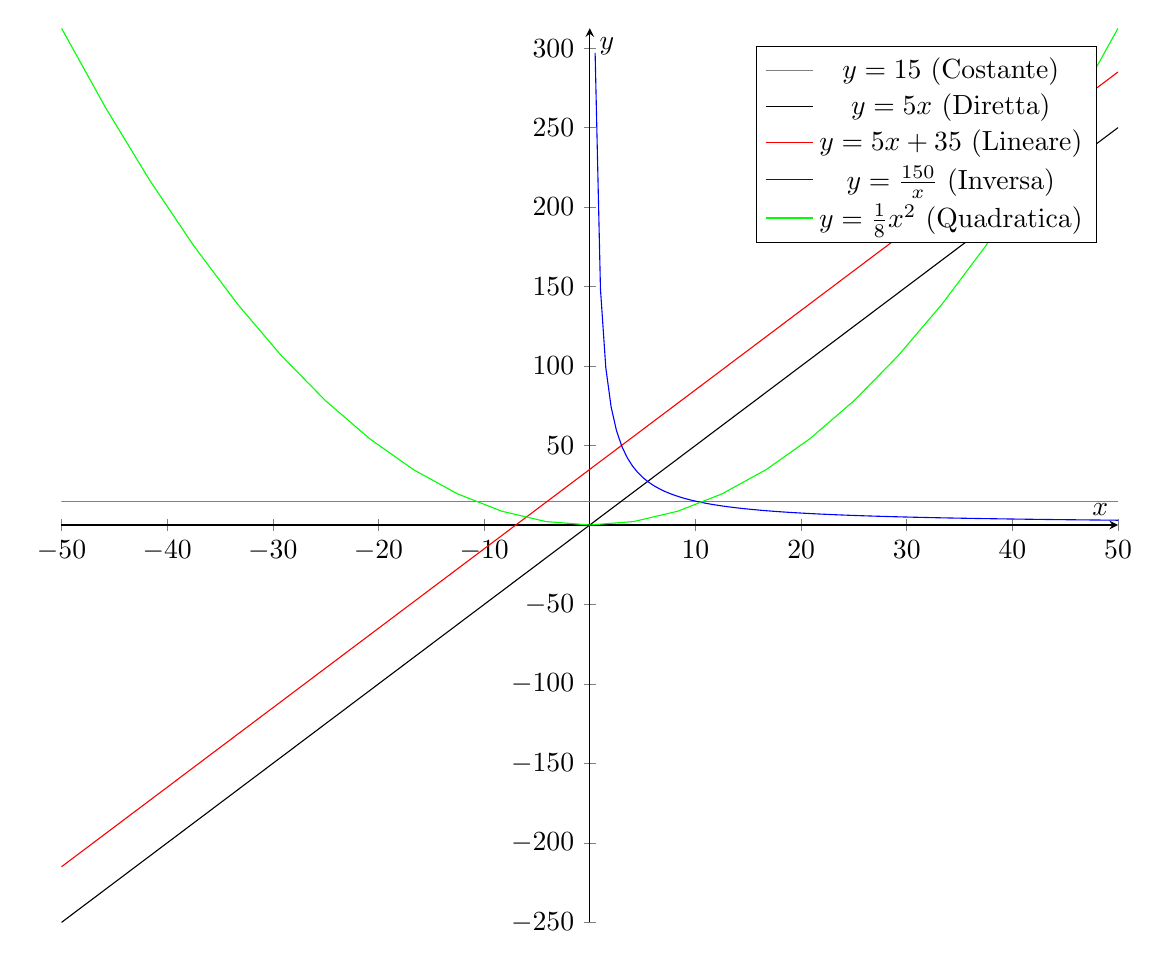
\begin{tikzpicture}
    \begin{axis}[
      axis lines = center,
      xlabel = \(x\),
      ylabel = \(y\),
    ]
      \addplot [
        domain=-50:50,
        color=gray,
      ]{15};
      \addlegendentry{\(y = 15\) (Costante)}

      \addplot [
        domain=-50:50,
        color=black,
      ]{5 * x};
      \addlegendentry{\(y = 5x\) (Diretta)}

      \addplot [
        domain=-50:50,
        color=red,
      ]{5 * x + 35};
      \addlegendentry{\(y = 5x + 35\) (Lineare)}

      \addplot [
        domain=0:50,
        color=blue,
        samples=100
      ]{150 / x};
      \addlegendentry{\(y = \frac{150}{x}\) (Inversa)}

      \addplot [
        domain=-50:50,
        color=green,
      ]{(1 / 8) * (x^2)};
      \addlegendentry{\(y = \frac{1}{8}x^2\) (Quadratica)}
    \end{axis}
    \end{tikzpicture}

    \pagebreak

    \subsubsection{Funzione Esponenziale}
    La funzione esponenziale e' quella funzione definibile come

    $$ y = k^x $$

    dove l'incognita e' quindi all'esponente. Tale funzione e' definita solo per valori 
    
    $$ k \in \mathbb{R}^+ - \{1\} $$

    ovvero $ k $ strettamente maggiore di $ 0 $ e diverso da $ 1 $ \small{(Se $ k = 1 $, allora $ y = 1^x $ percio' uguale a $ 1 $, ovvero una funzione costante)}.

    \begin{tikzpicture}
    \begin{axis}[
      axis lines = center,
      xlabel = \(x\),
      ylabel = \(y\),
    ]
      \addplot [
        domain=-3:3,
        color=red,
        samples=200,
      ]{2^x};
      \addlegendentry{\(y = k^x\) con \(k > 1\)}

      \addplot [
        domain=-3:3,
        color=blue,
        samples=200
      ]{(1 / 2)^x};
      \addlegendentry{\(y = k^x\) con \(0 < k < 1\)}
    \end{axis}
    \end{tikzpicture}
  }

  Caratteristiche:
  \begin{itemize}
    \item \textbf{Asintoto}: tendenza della funzione di avvicinarsi ad un valore senza mai raggiungerlo
    \begin{quote}
      $ k > 1 $, la funzione presenta un asintoto sull'asse $ x $ per $ x $ che tende a $ -\infty $, vedi curva rossa

      $ 0 < k < 1 $, la funzione presenta un'asintoto sull'asse $ x $ per $ x $ che tende a $ +\infty $, vedi curva blu
    \end{quote}
    \item \textbf{Punti notevoli}
    \begin{quote}
      $ (0,1) $, la funzione esponenzione passa sempre per $ y = 1 $ per $ x = 0 $

      $ (1,k) $, la funzione esponenziale ha sempre valore $ k $ per $ x = 1 $
    \end{quote}
  \end{itemize}

  \pagebreak

  \subsection{Equazione Esponenziale}
  Un'equazione esponenziale e' quella che ha almeno una incognita sull'esponente. La risoluzione e' immediata usando le regole delle potenze, vedi paragrafo precedente, e riportando tutto alla stessa base.

  Esempio:

  $$ 2^{3x - 5} = 8 $$
  $$ 2^{3x - 5} = 2^3 $$

  \quote{da qui si puo' passare al livello degli esponenti}

  $$ 3x - 5 = 3 $$
  $$ 3x = 3 + 5 $$
  $$ 3x = 8 $$
  $$ x = \frac{8}{3} $$
\end{document}
